\section{The purpose}
The purpose of this master thesis is to analyze methods for defining quotient types in Coq since there is no built-in method for implementing such constructions in this programming language. We seek ways to define quotient-like types similar to quotient types, where elements are considered equal if and only if they are in a quotient-defining relation. We will focus on quotient types with a normalization function and provide examples without a computable normalization function. For this purpose, we will use methods such as subtyping, inductive types based on traces of normalization functions, and more.

\section{Prerequisites}
This thesis assumes basic knowledge of algebraic concepts such as modular groups, fractions, and the Euclidean algorithm. More advanced constructions will be defined, like dividing sets by equivalence relations. The main focus is the Coq language, so basic knowledge of this programming language is necessary. The reader should be able to write definitions in Coq and differentiate between \mcoq{Fixpoint} and \mcoq{Definition}. Understanding how the termination checker works or knowing the sort hierarchy can aid in understanding this thesis fully, but it is optional. The reader is also expected to know the basic concepts of Type Theory, such as the product and sum of types. Additionally, optional sections include category theory and homotopy-type theory concepts. Any advanced construction from those fields needed to comprehend these sections will be defined in this thesis.

\section{Coq as a proof assistant}
Coq is a formal proof management system released under the GNU LGPL license. It was first introduced in 1984 and was based on the Calculus of Constructions, which relied on Type Theory. In 1991, Coq began using the more advanced Calculus of Inductive Constructions \cite{coqDoc} \cite{cicOrigins}, which supports higher-order logic, dependent types, and statically typed programming, among other features, all thanks to the Curry-Howard isomorphism \cite{curry-howard}.

Coq can perform simple computations. However, it was primarily developed for program extraction. Users can use functions proven in Coq in other programming languages, such as OCaml. In the Coq type system, every term has its type, and every type has its sort. This is an essential concept, as different sorts serve different purposes. There are four important sorts:

\begin{description}
\item[\mcoq{Prop}] -- intends to be the sort of logical prepositions. This sort is impredicative, which means propositions can quantify over all propositions. Imprecativity allows us to write propositions that say something about all propositions. Elements of this sort are removed during code extraction. Consequently, there are limitations on eliminating proofs of prepositions during type construction.

\item[\mcoq{SProp}] -- similar to \mcoq{Prop}, this sort is also intended to contain logical prepositions. The main difference is the definitional irrelevance of propositions. Irrelevance means that proofs of the same preposition in this sort are, by definition, equal.

\item[\mcoq{Set}] -- intends to be a sort for small types, like boolean values or natural numbers, but also products, subsets, and function types over these data types. Elements of this sort are expected to be preserved during code extraction. Accordingly, computations should take place in this sort.

\item[\mcoq{Type}] -- contains small and large sets like \mcoq{Prop} and \mcoq{Set}. Therefore, every type and sort lives in \mcoq{Type}, for example, \mcoq{Prop : Type}.
\end{description}

\begin{coq}{Hierarchy of sorts}{xoq:universes}
 More experienced readers might notice that this definition of \mcoq{Type} seems wrong. We know only sorts at the bottom of the hierarchy can contain itself \cite{TypeNotInType}. \mcoq{Type} is not \mcoq{Prop} but it contains \mcoq{Prop}, therefore it not at the bottom of hierarchy. Despite this, when Coq is asked what is the type of \mcoq{Type}, it answers \mcoq{Type : Type}. In reality, there is a whole infinite hierarchy of sorts in Coq, and every \mcoq{Type} has its level, which is just hidden from users for convenience. Therefore, \mcoq{Type : Type} should be read as \mcoq{Type(n) : Type(n+1)}.
\end{coq}

Coq allows users to define only functions that terminate. For many simple functions, the termination checker automatically deduces that the function terminates. However, sometimes it requires much work to convince it. The other consequence of this is the fact that in Coq, reasoning about partial functions is difficult. Nevertheless, later we will learn how to represent non-terminating computations. The most significant advantage of Coq is that it has an imperative tactic language, which makes proving theorems much more accessible than in languages like Agda \cite{agda} or Idris \cite{idris}.

\section{Quotient types}
Quotient type is a concept from abstract algebra \cite{AbstractAlgebra}, which has found applications in other fields like computer science.
\begin{defi}{Quotients in abstract algebra}{def:quotients_in_aa}
In abstract algebra, an underlying set $T$ partitioned by equivalence relation ($\sim$) is called a \emph{quotient} and denoted as $T/\sim$.
\end{defi}
\begin{example}{Clock operations}{ex:clock}
An excellent example of a quotient is an analog clock, more precisely, the sequence of consecutive hours on it. The operations on the clock can be modeled by operations in additive integer group modulo 12 (we denote it as $\mathbb{Z}_{12}$). Almost everyone has experience with time tracking, and it is not surprising that after 12 o'clock, there is 1 o'clock. This phenomenon is caused by the fact that numbers 1 and 13 both give the same remainder when divided by 12 and that is why they are equivalent in the context of time tracking.
$$\ldots \equiv -11 \equiv 1 \equiv 13 \equiv 25 \equiv 37 \equiv \ldots \; (\textrm{mod } 12) $$
As expected, 1:00 and 13:00 are the same on an analog clock.
\end{example}

\subsection{The equivalence relation}
In order to formalize quotient types, first, we need to define equivalence relations and check their properties.

\begin{defi}{Equivalence relation}{def:equiv_rel}
\begin{minted}{coq}
Class equivalance_relation {A : Type} (R : A -> A -> Prop) := {
  equiv_refl  : forall x : A, R x x;
  equiv_sym   : forall x y : A, R x y -> R y x;
  equiv_trans : forall x y z : A, R x y -> R y z -> R x z;
}.
\end{minted}
\end{defi}
\begin{coq}{Class}{coq:class}
In Coq \mcoq{Class} is a keyword defining typeclasses known, for example, from Haskell \cite{Haskell}. They are used for defining interfaces for types. For someone unfamiliar with the concept of typeclasses, it can be considered as a classical Coq \mcoq{Definition} with a slightly more user-friendly application.
\end{coq}

Equivalence relation (defined in \ref{def:equiv_rel}) is a generalization of the most fundamental relation: equality. Similarly, we want every element to be equivalent to itself. This property is called \emph{reflexivity}. Moreover, we want this relation to be \emph{symmetric}, which means that ($a \sim b$) is equivalent to ($b \sim a$). The last property is \emph{transitivity}. For symmetric relations, it says that when two elements, a and b, are both equivalent to a third one, then a is equivalent to b. Relations with those three properties induce equivalence classes \cite{AbstractAlgebra} over the underlying set.

\begin{defi}{Equivalence class}{def:equiv_class}
For an underlying set T and an equivalence relation ($\sim$), the set of all elements equivalent to $a \in T$ is called \emph{equivalence class} and denoted as $[a]_\sim$.
$$ [a]_\sim = \{x \in T : x \sim a \}$$
A quotient $T / \sim$ is a set of all equivalence classes. 
$$ (T / \sim) = \{[t]_\sim : t \in T\}$$
\end{defi}

\begin{example}{Fraction's notations}{ex:frac_equiv}
An example of a set with an equivalence relation is the set of fraction's notations. We know that every fraction can be represented in infinitely many ways. Therefore, we can define the equivalence relation in which all representations of the same fraction.
$$ \frac{1}{2} = \frac{2}{4} = \frac{3}{6} = \frac{4}{8} = \frac{5}{10} = \dots$$
\end{example}

\begin{example}{Modular arithmetic}{ex:mod_equiv}
Another example is a modular group from Example \ref{ex:clock}. We showed that multiple integers have the same value in modular arithmetic. Hence, all numbers with the same value are in the same equivalence class.
$$ \dots \equiv -11 \equiv 1 \equiv 13 \equiv 25 \equiv 37 \equiv \dots (\textrm{mod } 12) $$
\end{example}
\begin{vis}[G]{Equivalence classes}{vis:equivalance_classes}
Visualization of equivalence classes for selected elements of group $\mathbb{Z}_{12}$. Lines represent elements in equivalence relation, and ellipses represent equivalence classes:
\begin{center}
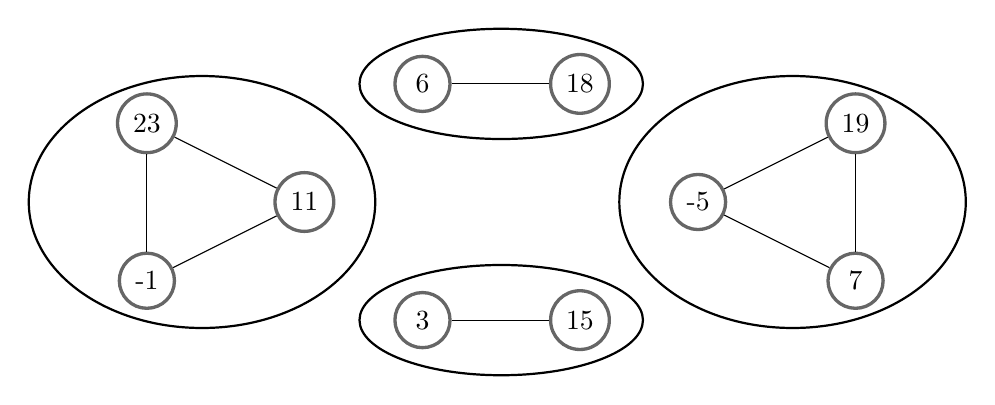
\begin{tikzpicture}[
    node/.style={circle, draw=black!60, very thick, minimum size=7mm},
    ]
    %Nodes
    \node[node] at (-0.5, 0.5) (a) {-1};
    \node[node] at (1.5, 1.5) (b) {11};
    \node[node] at (-0.5, 2.5) (c) {23};
    \node[node] at (6.5, 1.5) (d) {-5};
    \node[node] at (8.5, 0.5) (e) {7};
    \node[node] at (8.5, 2.5) (f) {19};
    \node[node] at (3, 0) (g) {3};
    \node[node] at (5, 0) (h) {15};
    \node[node] at (3, 3) (i) {6};
    \node[node] at (5, 3) (j) {18};
    
    %Lines
    \draw[-] (a) -- (b);
    \draw[-] (a) -- (c);
    \draw[-] (b) -- (c);
    \draw[-] (d) -- (e);
    \draw[-] (d) -- (f);
    \draw[-] (e) -- (f);
    \draw[-] (g) -- (h);
    \draw[-] (i) -- (j);
    
    %elipses
    \draw[thick] (4,0) ellipse (1.8 and 0.7);
    \draw[thick] (4,3) ellipse (1.8 and 0.7);
    \draw[thick] (0.2,1.5) ellipse (2.2 and 1.6);
    \draw[thick] (7.7,1.5) ellipse (2.2 and 1.6);
\end{tikzpicture}
\end{center}
\end{vis}

\subsection{Type-theoretic view}
This thesis focuses on the implementation of quotient types in Coq. Thus, we focus on this concept from the type theory perspective. In type theory, quotient types are also induced by some equivalence relation ($\sim$) on underlying type $T$ and denoted as $T/\sim$. We denote the equality of elements in the quotient type $T/\sim$ as $a =_\sim b$. Two elements $a$ and $b$ are equal ($a =_\sim b$) if and only if they are in the relation ($a \sim b$). Every element of the underlying type $T$ is also an element of quotient type $T/\sim$.

Nevertheless, only some functions from underlying type $T$ are well-defined from type $T/\sim$. Function $f : T \rightarrow X$ defined on the underlying types is also a well-defined function $f : (T/\sim) \rightarrow X$ on the quotient type, if $a \sim b$ implies that $f(a) = f(b)$. Without this restriction, we could differentiate between elements of the same equivalence class by applying an ill-defined function. In other words, applying an ill-defined function breaks the rule that says: $x = y \Rightarrow f(x) = f(y)$.

\section{Quotient types in Coq}
As we mentioned previously, Coq has no built-in method for quotient constructions. Nevertheless, quotients are a helpful concept in formalizing mathematics. Moreover, quotient data types such as sets and multisets are used in many algorithms. Therefore, since Coq was introduced, users have been looking for ways to deal with quotients in the Coq language \cite{cicQuotient} \cite{PragmaticQT} \cite{NormalizedTypes}. From those studies, two ways of working with quotient-like types emerged. The first one focuses on replacing the equality relation with an equivalence relation. The second focuses on changing the underlying type so that equivalence implies equality. Both approaches have their disadvantages and both are used depending on the situation. In this paper, we focus on the second approach.

\subsection{The setoid approach}
\begin{defi}{Setoid}{def:setoid}
In mathematics, a \emph{setoid} is a set $A$ with an equivalence relation ($\sim$). It is denoted as $(A, \sim)$. In setoids, relation ($\sim$) is meant to be used in place of equality on set A.
\end{defi}
Setoids are concepts known from type theory \cite{SetoidsInTT} \cite{Setoids2}. In Coq, they are often used in the formalization of mathematical concepts. When working with setoids, we need to replace the equality relation in the theorem we are proving with the equivalence relation of the setoid we want to use. It is a minor inconvenience. The bigger one occurs when we want to apply a function on an element of our setoid. In this case, we must prove that the applied function is well-defined on setoid (respects equivalence relation). The Coq standard library has tools to help users use setoids, like rewriting parts of equivalent statements. Unfortunately, it is still far more problematic than using simple equality.

\subsection{The quotient-like type approach}
Another approach to the lack of quotients in Coq is to define quotient-like types where equivalence is the same as equality. This approach usually involves reducing each equivalence class to a single element.

\subsubsection{Subtyping}
This concept will be discussed later in Chapter 2, so the formal definition will be skipped here. Its main idea is to construct a type containing a specific subset of elements. Those elements need to satisfy a particular predicate in the case of the quotient -- the predicate of being normalized.

\subsubsection{A tailor-made inductive type}
This approach usually gives the best results but only applies to some quotient types. Chapter 4 will show examples of such types based on traces of normalization function. Unfortunately, no general way of defining such type out of the normalization process has been found.

\subsubsection{Additional axioms}
To the Coq system, we can add axioms, and by doing so, we can define quotients similarly as in other languages like Lean \cite{lean4}. This particular construction will be shown in Chapter 6. Unfortunately, by adding axioms, we lose the computability of our proofs. However, usually, we do not need computable proofs. Moreover, it's essential to exercise caution to avoid introducing contradictions into the system.
\begin{example}{}{ex:ill_defined_mod2}
When dealing with arithmetic modulo 2, we might be tempted to add the following axiom:
\begin{minted}{coq}
Axiom Modulo2 : forall n: nat, n = S (S n).
\end{minted}
It lets us effortlessly rewrite numbers back to their normalized form. Nevertheless, by mistake, we introduced a contradiction. Let us define a function \mcoq{isZero}, which returns \mcoq{true} for zero and only zero. Therefore \mcoq{true = isZero(0) = } \\ \mcoq{isZero(2) = false}, since \mcoq{0 = 2}.
\end{example}

\subsubsection{Private inductive types}
Another way to construct quotients is by using private inductive types \cite{PrivetInductive}. By using them, we can define the type on which pattern matching outside the module where it is defined is forbidden. If it is done correctly, it enables us to create constructions like in Example \ref{ex:ill_defined_mod2} without introducing contradiction since a user cannot define ill-defined functions.

\section{The equivalence relation induced by a function}
\begin{theo}{The equivalence relation induced by a function}{th:equiv_by_fun}
Every function $h: T \rightarrow B$ induces a specific equivalence relation ($\sim_h$) defined below:
$$ \forall x, y \in T, x \sim_h y \iff h(x) = h(y). $$
Moreover, every function $g: B \rightarrow X$ induces a well-defined function $f : T/\sim_h \rightarrow X$ defined as $f = g \circ h$. 
\end{theo}

\begin{proof}{The equivalence relation induced by a function}{proof:equiv_by_fun}
Proof that ($\sim_h$) is an equivalence relation follows directly from the fact that equality on type $B$ is an equivalence relation. \qed \\ 
Given $a, b \in T$ such that $a \sim_h b$. By definition of ($\sim_h$) we know that $h(a) = h(b)$ therefore $f(a) = g(h(a)) = g(h(b)) = f(b)$. So $f$ respects relation $\sim_h$. \qed
\end{proof}
\subsection{Definition of a normalization function}
This paper focuses on the particular case of the function $h: T \rightarrow T$, which is idempotent. Such functions we call normalization functions.
\begin{defi}{Normalization function}{def:normalization_function}
\begin{minted}{coq}
Class normalization {A : Type} (f : A -> A) := 
  idempotent : forall x : A, f (f x) = f x.
\end{minted}
\end{defi}
As we know, equivalence relations partition elements into equivalence classes. A normalization function selects a single element from each equivalence class. Elements that have been selected are referred to as normalized or elements in normal form. The idempotence restriction is required to ensure that the normalization function does not change elements that are already in normal form.

\begin{vis}[B]{Normalization function}{vis:normalization_fuction}
Example of applying normalization function to rational numbers represented as $\mathbb{Z} \times \mathbb{N_+}$:
\begin{center}
    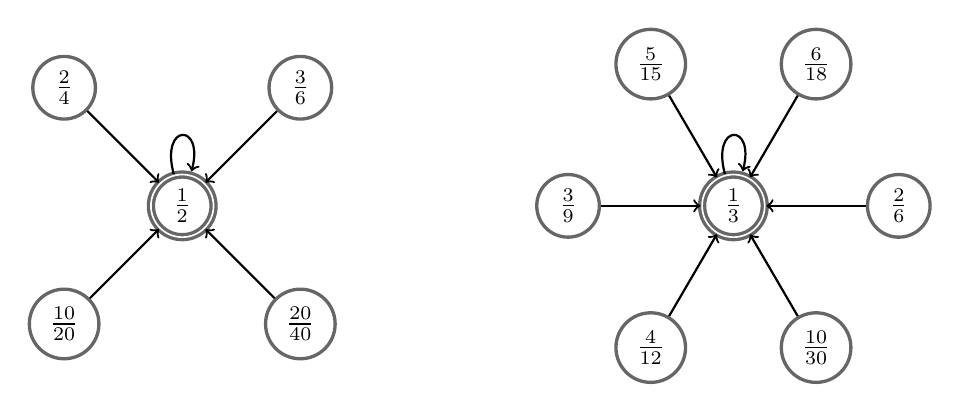
\begin{tikzpicture}[
    node/.style={circle, draw=black!60, very thick, minimum size=0.4}
    ]
    
    %Nodes
    \node[node, double] at (2, 2) (a) {$\frac{1}{2}$};
    \node[node] at (0.5, 3.5) (a0) {$\frac{2}{4}$};
    \node[node] at (3.5, 3.5) (a1) {$\frac{3}{6}$};
    \node[node] at (0.5, 0.5) (a2) {$\frac{10}{20}$};
    \node[node] at (3.5, 0.5) (a3) {$\frac{20}{40}$};

    \node[node, double] at (9, 2) (b) {$\frac{1}{3}$};
    \node[node] at (11.1, 2) (b1) {$\frac{2}{6}$};
    \node[node] at (6.9, 2) (b2) {$\frac{3}{9}$};
    \node[node] at (7.95, 0.2) (b3) {$\frac{4}{12}$};
    \node[node] at (7.95, 3.8) (b4) {$\frac{5}{15}$};
    \node[node] at (10.05, 0.2) (b5) {$\frac{10}{30}$};
    \node[node] at (10.05, 3.8) (b6) {$\frac{6}{18}$};
    
    %Lines
    \path[->, thick] (a) edge [loop above] node {} (a);
    \draw[->, thick] (a0) -- (a);
    \draw[->, thick] (a1) -- (a);
    \draw[->, thick] (a2) -- (a);
    \draw[->, thick] (a3) -- (a);
    
    \path[->, thick] (b) edge [loop above] node {} (b);
    \draw[->, thick] (b1) -- (b);
    \draw[->, thick] (b2) -- (b);
    \draw[->, thick] (b3) -- (b);
    \draw[->, thick] (b4) -- (b);
    \draw[->, thick] (b5) -- (b);
    \draw[->, thick] (b6) -- (b);
    \end{tikzpicture}
\end{center}
\end{vis}

\subsection{Examples of normalization functions}
\begin{example}{Rational numbers}{ex:normalization_fractions}
The standard representation of rational numbers is $\mathbb{Z} \times \mathbb{N}$. For such representation, we can define elements in normal form as irreducible fractions. Therefore, the normalization function should reduce the fraction by dividing the numerator and the denominator by their greatest common divisor.
\end{example}
\begin{example}{Unordered pair}{ex:normalization_unordered_pirs}
We can define a normalization function for unordered pairs using linear order defined for the underlying type, for example, pairs of natural numbers. Such a function uses the linear order to sort elements of a pair. By doing so, the original order of elements in the pair is lost.
\end{example}
\begin{example}{Integers modulo $n$}{ex:normalization_mod}
The normalization function for numbers in arithmetic modulo $n$ is as we expect the operation of calculating modulo.
\end{example}

\section{Quotient types without a normalization function}
Normalization functions are an excellent tool for defining quotient-like types. By using them, we can select a representative for each equivalence class. Unfortunately, not every quotient type has a computable normalization function. With the axiom of choice, we can always select a set of representatives of each equivalence relation. Therefore, we can always define the normalization function. However, in this thesis, we try to avoid utilizing additional axioms, since they make functions uncomputable.

\subsection{Unordered pairs}
An unordered pair is one of the most basic quotients for which a normalization function does not exist. A normalization function exists if an underlying type has a decidable linear order. However, in the general case, it is impossible to define the normalization function. Moreover, for some types like, for example, $\mathbb{N} \rightarrow \mathbb{N}$, it is also possible to create such a normalization function based on the computable minimum and maximum, although linear order is not decidable \cite{DefinableQuotients}.
\pagebreak
\begin{theo}{}{th:no_normalization_for_unordered_pair}
There is no function $f: (A \times A) \rightarrow A \times A$ for any type A that, for any $\medcircle , \square \in A$ we have $f((\medcircle , \square)) = f((\square, \medcircle))$ and $\medcircle , \square \in f((\medcircle , \square))$ 
\end{theo}

\begin{proof}{}{proof:no_normalization_for_unordered_pair}
Since $f$ is a function for every type $A$, we cannot use values of $\square, \medcircle$ to determine the order of elements. Therefore, there are only two functions: $f((\medcircle , \square)) = (\medcircle , \square)$ and $f((\medcircle , \square)) = (\square , \medcircle)$, that satisfy the second property. As can be easily checked, neither of them satisfies the first property. \qed
\end{proof}

\subsection{Real numbers represented by Cauchy’s sequences}
\begin{defi}{Cauchy sequance}{def:cauchy_seq}
Sequence $\{a_n\}_{n\in \mathbb{N}}$ in called \emph{Cauchy sequance} if elements become arbitrarily close to each other as the sequence progresses \cite{Anal}.
$$
    (\forall \epsilon > 0). \; (\exists N \in \mathbb{N}^+). \; (\forall m, n > N). \; |a_n - a_m| < \epsilon
$$
\end{defi}
Cauchy sequences are often used to construct real numbers out of rational numbers \cite{CauchyReals}. The issue with this construction is that infinitely (even uncountably) many sequences represent a single real number. Using quotients to fix this problem would give us an excellent representation of real numbers. Unfortunately, there is no computable normalization function for Cauchy sequences.

\begin{theo}{}{th:no_normalization_for_reals}
There is no computable function $f: (\overline{\mathbb{N} \rightarrow \mathbb{Q}}) \rightarrow (\overline{\mathbb{N} \rightarrow \mathbb{Q}})$, where $(\overline{\mathbb{N} \rightarrow \mathbb{Q}})$ means computable function. Such that, for any $a, b \in (\overline{\mathbb{N} \rightarrow \mathbb{Q}})$ we have $\lim_{n \rightarrow \infty}a_n = \lim_{n \rightarrow \infty}b_n \iff f(a) = f(b)$.
\end{theo}

\begin{proof}[G]{}{proof:no_normalization_for_reals}
Let's assume such function $f$ exists.
Let $s_k$ be a sequence consisting of ones to $k$-th place and zeros after. Let $s_\infty$ be a sequence consisting of all ones. \\For all $k$ limit of $s_k$ is zero, and limit of $s_\infty$ is one. Therefore $f(s_k)  \neq f(s_\infty)$. If they are different, that means there is a number $t \in \mathbb{N}$ for which $f(s_k)_t  \neq f(s_\infty)_t$. So, we are able to differentiate between those two in finite time.\\
Let $M$ be the initial state of the universal Turing machine. Let $c_M(t)$ be zero if the Turing machine halts before $t$-th step and one otherwise. This function is computable for every $M$, so we can apply a function $f$ to it and check if the Turing machine with initial state $M$ halts. But the halting problem is undecidable \cite{Undecidable}, so such function $f$ cannot exist. \contradiction
\end{proof}

\subsection{The delay monad}
\begin{defi}{Delay monad}{def:delay_monad}
\begin{minted}{coq}
CoInductive delay (A : Type) : Type := 
| output : A -> delay A
| wait   : delay A -> delay A.
\end{minted}
\end{defi}
The delay monad \cite{DelayedMonad} represents computations that may or may not terminate. It is a valuable concept in Coq since it provides an entirely safe way of implementing functions that may not terminate. We want our normalization function to return a value immediately if the computation ever terminates and return infinite delay otherwise. Unfortunately, similar to Cauchy sequences, such a normalization function does not exist.
\begin{theo}{}{th:no_normalization_for_delay_monad}
There is no computable function $f: \textrm{delay} \; A \rightarrow (A + \textrm{unit})$ that, for any terminating computation, returns its final value. Otherwise, it returns an element of unit type.
\end{theo}
\begin{proof}{}{proof:no_normalization_for_delay_monad}
Let's assume that such function $f$ exists. We can model the computation of every partial computable function using a delay monad. Using the normalization function $f$, we can determine if a partial function terminates. This makes the halting problem decidable, but we know it is undecidable \cite{Undecidable}. Therefore, such a normalization function cannot exist. \contradiction
\end{proof}
